This chapter describes the multi-view clustering approach proposed by this thesis. The approach consists of four main steps. First, we extract the code fragments that we intend to cluster. Next, these code fragments are enriched with static, semantic and dynamic information and used to construct a graph. In this graph, the edges and their weight are determined by the information streams we consider. The graph is subsequently partitioned into a suitable set of clusters. The final step measures the quality of the resulting decomposition. In the next sections, we further discuss each step of the approach.

\section{Notation}
Before diving into the details of the approach, we introduce some notation to help the reader navigate through the sections. \par

\begin{itemize}
    \item[$M$] A monolithic project is a quadruple $M = (CF_M, S_M, L_M, D_M)$, where $CF_M$ is the set of code fragments, $S_M$ the set of static dependencies, $L_M$ the set of lexical dependencies\footnote{A lexical dependency indicates that two code fragments embed similar domain terms in their source code and therefore are related to each other. Since this does not mean that they directly depend on each other, one could argue to call it a dependency. However, for simplicity, we decided to refer to this relationship as a dependency in the rest of this thesis.}, and $D_M$ the set of dynamic dependencies. The lexical dependencies are often referred to as semantic dependencies. The terms have the same meaning and are used interchangeably in this report.
    \item[$CF_M$] A $CF_M$ is the set of code fragments extracted from the code base of monolith $M$. Each code fragment $cf_k \in CF_M$ implements some functionality and has the following properties: name $(name_k)$, type $(type_k)$, file path $(path_k)$, source code $(code_k)$, and a boolean $(clustered_k)$ that decides whether the code fragment is clustered. These properties are further discussed in Section \ref{s:step1_cf_extraction}. Each code fragment is also enriched static dependencies $s_k \in S_M$, lexical dependencies $l_k \in L_M$ and dynamic dependencies $d_k \in D_M$.
    \item[$S_M$] The set of static dependencies extracted from monolith $M$. Each static dependency $s_k \in S_M$ is represented as a triple $s_k = (caller, callee, weight)$, where the caller calls the callee. The caller and callee represent top-level code fragments. The weight of a static dependency from $cf_i$ to $cf_j$ is determined by taking the union over the set of static dependencies from all its descendants. E.g. if two nested methods defined inside $cf_i$ have a static dependency to $cf_j$, we obtain the following static dependency: $s_k = (cf_i, cf_j, 2)$.
    \item[$L_M$] The set of lexical dependencies $l_k \in L_M$ extracted from monolith $M$. Each lexical dependency represents a triple $l_k = (cf_i, cf_j, weight)$ where $cf_i$ and $cf_j$ are top-level code fragments that share at least one lexical term. The lexical terms are extracted from the source code of the corresponding code fragment. The weight is determined by the tf-idf weight of each pair of overlapping terms. This is further explained in Section \ref{ss:semantic_dependencies}.
    \item[$D_M$] The set of dynamic dependencies belonging to monolith $M$. Like with static dependencies, each dynamic dependency $d_k \in D_M$ is a triple where the first element is the caller, the second element the callee, and the third element the weight. The weight in the dynamic dependency is determined by the frequency of the calling relation.
    \item[$Service_M$] The set of microservices obtained from monolith $M$ where each $service_k$ contains a subset of the top-level code fragments $service_k \subseteq CF_M$.
\end{itemize}

\section{Step 1: Code fragment extraction}\label{s:step1_cf_extraction}
The first step of our approach is to extract the set of code fragments $CF_M$ that are available in monolithic project $M$. As mentioned before, a code fragment can represent a module, class, method or function. 
In order to collect code fragments, we first collect the set of '.py' files related to monolith $M$. We do this by recursively walking over the main source (often called 'src') folder of the project. Each '.py' file that we find, we parse into an Abstract Syntax Tree (AST). The AST is a tree representing the syntactic structure of code. To obtain the AST, we use Python's standard ast\footnote{\href{https://docs.python.org/3/library/ast.html}{https://docs.python.org/3/library/ast.html}} library, which makes it easy to parse code into an AST and analyse it.
We then walk over each of the elements in the AST and when the element represents a 'method', 'function', 'class', or 'module', we create a new code fragment $cf_k$. The discovered code fragments are enriched with the following information.

\begin{itemize}
    \item \textbf{Id.} The id of the code fragment. The id is a composed of 'cf' and a global counter. For example, the first discovered code fragment gets the id 'cf1'.
    \item \textbf{Name.} The name of code fragment $cf_k$ is constructed by taking its fully qualified name. The fully qualified name is unambiguous in the sense that it includes all names of the hierarchical sequence above the given element and the name of the element itself. This way we can always identify the location of the code fragment. For example, the name of class $Person$ defined inside module $person.py$ that is located in the  $src$ folder of the program becomes: $src.person.Person$. The name always starts with the main folder in which all the source files are located.
    \item \textbf{Type.} The type of the code fragment, where the type is either a module, class, function or method. Methods are similar to functions but are defined inside classes while functions are not. The type of a code fragment is determined by looking at the abstract syntax derived from the AST. Since functions and methods are both classified under the same abstract syntax, we distinguish them by looking at the 'self' input parameter. The 'self' input parameters indicates the definitions uses an instance of the object, which means that the code fragment has to be a method. We are aware that this is not a watertight implementation, as 'self' is only a widely used naming convention and can be called differently. For this reason, we also look if the code fragment is defined in a class or not. This because methods have to be defined inside a class. 
    \item \textbf{File path.} The file path ($path_k$) of the file in which the code fragment is defined. 
    \item \textbf{Code.} The source code ($code_k$) of the code fragment in the form of text. The code is necessary to extract lexicons and determine semantic dependencies between code fragments.
    \item \textbf{Start lineno.} This is an integer value that represents the line number at which the code fragment starts.
    \item \textbf{End lineno.} Similar as the one before, but then indicating the end of a code fragment. This start and end line number of the code fragment are important in a later stadium where we want to identify code fragments based on the file path and line number.
    \item \textbf{Input params.} The set input parameters of the code fragments represented. The input parameters are represented by its name, and thus not the type. The input parameters are necessary to compute the quality metric Cohesion at Message level (CHM), which is further explained in Section \ref{s:quality_computation}.
    \item \textbf{Output params.} The names of the returning parameters of the code fragment. Also this property is necessary for the computation of CHM.
    \item \textbf{Defined in.} This property shows the top-level code fragment to which a lower-level code fragment belongs. For top-level code fragments, this property will be empty. To illustrate this better, suppose we have a method $X$ ($cf_i$) defined inside class $Y$ ($cf_j$). The 'defined in' property for code fragment $cf_i$ will refer to code fragment $cf_j$. This information is necessary to cluster on the right level of granularity. 
    \item \textbf{Nested code fragments.} This last property gives all nested code fragments, where each code fragment is represented by its 'name' property. 
\end{itemize}

The set of code fragments $CF_M$ together with its properties extracted from monolith $M$ are exported to a JSON file. We do this for two reasons. At first, intermediate results make it easier to reproduce the results of the research. In addition, the exported data eased the process of verifying the correctness of the tool. The tool is verified in Chapter \ref{c:verification} of this thesis.
    
\subsection{Level of cluster abstraction}\label{ss:level_of_cluster_abstraction}
There are different levels of abstraction in which we can cluster the code base. Most of the related approaches found in the literature review work with Java systems and cluster on class level. However, unlike Java, Python files can also contain definitions that are defined outside the scope of a class (like functions). This means that when we cluster on class-level, definitions defined outside classes are not considered. To deal with this, we could either incorporate each individual function into the clustering or group functions to its member module. \par
Clustering each individual function results in a very fine grained clustering. However, being this fine grained brings some additional challenges. At first, it will increase the number of possible decompositions which makes the search process for the optimal decomposition harder. Secondly, when clustering individual functions, it is more likely that we obtain no information about the function. For example, when a function does not have any structural dependencies, we are unable to cluster it when only employing static analysis. However, when the function is grouped to its member module, it can still be clustered when other functions in its module do have some static dependencies. \par
As a solution, we could choose to assign functions to its member module. This is similar to linking methods to its member classes. Methods are linked to classes since they have some relation with each other. The same holds for functions that are written in the same module. The developer groups functions in the same module with the rationale that the code is related to each other. Grouping code into modules makes the code logically organised and is therefore easier to understand and use. \par
We decided to group functions to its member module in our approach. The reason for this is based on the assumption that the functions inside a module implement related code and therefore should never be split from each other. This is the same rationale as related approaches use for grouping member methods with their classes. 

\section{Step 2: Feature extraction}\label{s:step2_features}
After we obtain the set of code fragments $CF_M$ of monolith $M$, we enrich them with static ($S_M$), semantic ($L_M$) and dynamic ($D_M$) edges that describe relations between code fragments. Each dependency is further explained in the next sections.

\subsection{Static dependencies}
The static dependencies $S_M$ are obtained by performing static analysis over monolith $M$. Static analysis means that the code is analysed as it is, and thus, without actually executing it. To collect the static dependencies, we generate a call graph in which calling relationships between code fragments are depicted. The creation of call graphs is out of context for this thesis and therefore we looked for a tool that has already been implemented.

\subsubsection{Selecting a call graph generator}\label{sss:call_graph_generators}
Python is a dynamic language which makes it hard to obtain certain dependencies. In dynamically typed languages, the type of objects (such as variables) are only known at runtime. This means that analysing plain source code does not reveal the types of objects. Let's illustrate this behaviour by an example. Suppose we have created a variable $a$ which represents an instance of the class $Customer$. When we use $a$ as input for an imaginary function $X$, we have to define a dependency from $x$ to $a$ without knowing what the type of $a$ is. This property among others makes it challenging for tools to get a complete picture of the existing structural dependencies. \par

To select the most appropriate call graph generator, we analysed each tool against a set of Static-analysis Criteria (SC). Each criterion is ordered by its priority. This means we start with the most important criteria and end with the least important ones. 

\begin{itemize}
    \item[\textbf{SC1}] \textbf{Freely available.} The tool must be open source and be freely in use. This means that commercial tools will not be considered. 
    \item[\textbf{SC2}] \textbf{Not deprecated.} It is important to us that the tool is not deprecated. This gives us a higher chance that the tool works considering that packages the tool is build upon might change.
    \item[\textbf{SC3}] \textbf{Support of higher-order functions.} One of Python's features is its support of higher-order functions. This means that functions can be assigned to variables, passed as parameters to other functions, or serve as return values \cite{salis15pycg}. Supporting higher-order functions is a challenging task in which many tools do not succeed. For this reason, we think it is a good discriminating criterion for selecting an appropriate call graph generator tool. 
\end{itemize}

Despite Python's increased popularity, surprisingly few tools have been introduced that generate call graphs \cite{salis15pycg}. A study by \citeauthor{yu2019empirical} \cite{yu2019empirical} compared three widely used static call graph tools to six open source projects. These tools are all frequently mentioned in developers communities and are Pyan \cite{fraser2018pyan3}, Code2flow \cite{rogowski2021code2flow} and Understand \cite{scitools2021understand}. Pyan parses the Abstract Syntax Tree (AST) to construct the call graph while Code2flow constructs the call graph at lexical level \cite{yu2019empirical}. Understand is a commercial tool to generate call graphs. A recent paper by \citeauthor{salis15pycg} \cite{salis15pycg} introduced a new technique, named PyCG, to generate call graphs that relies on inter-procedural analysis. The tool compared itself with Pyan \cite{fraser2018pyan3} and Depends \cite{zhang2018depends}. Depends is another call graph generator that infers syntactical relations among source code entities, such as files and methods. However, both Pyan and Depends do not perform well with higher-order languages such as Python as functions that are assigned to variables or passed to other functions are not captured \cite{salis15pycg}. \par
The tools that are analysed in Table \ref{tab:analysis_of_call_graph_generators} are found by an extensive search on the internet. All the considered call graph generators are implemented for Python code. We also looked into call graph generators used by related approaches found during the literature review (see Table \ref{tab:reviewed_papers}). There is only one related technique that analyses the structural dependencies specific for Python application. This is the approach proposed by \citeauthor{matias2020determining} \cite{matias2020determining}. However, their approach does not rely on a call graph generator tool as they collect the structural dependencies themselves by analysing the abstract syntax tree. The code they used for this is publicly available on their Github, but not applicable for us since it limits itself to applications that use the Django web framework. 

\begin{table}[h]
    \small
    \caption[Analysis of call-graph generators for Python]{Analysis of call-graph generators for Python. Each column in the table represents a Static-analysis Criteria (SC) explained in Section \ref{sss:call_graph_generators}. A cross (x) indicates that the criteria is meet while a stripe (-) indicates the opposite. When the information is not available we put N/A.}\label{tab:analysis_of_call_graph_generators}
    \begin{tabular}{>{\raggedright}m{100pt}>{\raggedright}m{25pt}>{\raggedright}m{25pt}>{\raggedright\arraybackslash}m{25pt}}
        \toprule
        Call-generator & SC1 & SC2 & SC3\\
        \midrule
        Understand \cite{scitools2021understand} & - & x & N/A \\
        \midrule
        PyCG \cite{salis15pycg} & x & x & x \\
        \midrule
        Depends \cite{zhang2018depends}& x & x & - \\
        \midrule
        Pyan \cite{fraser2018pyan3} & x & - & - \\
        \midrule
        Code2flow \cite{rogowski2021code2flow} & x & - & x\\
        \bottomrule
    \end{tabular}
\end{table}

The analysis shows that PyCG \cite{salis15pycg} is the most suitable tool. The author of PyCG also compared the tool to Depends and Pyan \cite{salis15pycg} and shows that PyCG outperforms them both in terms of completeness and soundness. A call graph is complete when it does not contain any edges that do not actually exists. This means that an incomplete call graph contains edges that should not be there. A sound call graph is realised when it contains every actual call edge. A call graph is unsound when it misses edges that should actually be there. Note that in our approach, being unsound is worse than being incomplete. \par

\subsubsection{Obtaining static dependencies}
The analysis of the call graph generators made us decide to work with PyCG. PyCG\footnote{\href{https://github.com/vitsalis/PyCG}{https://github.com/vitsalis/PyCG}} is implemented in Python and is freely available on GitHub. After executing PyCG on the selected monolith $M$ project, call edges $s_k \in S_M$ are derived from it and linked to its corresponding code fragment identified in the previous step (see Section \ref{s:step1_cf_extraction}). A limitation that we discovered when implementing PyCG in our tool is that it does not take into account the frequency of calls. This means, for example, when function $X$ calls for function $Y$ three times, only a single dependency will be noted. Counting the frequency of calls would be valuable information for our analysis, as it says something about the strength of a dependency, where a higher frequency indicates a stronger dependency. However, since we found this out after analysing the call graph generator tools, we did not consider it as a selection criteria. \par
The static dependencies for top-level code fragments represent the sum of its member code fragments together with its own dependencies. When looking at Listing \ref{lst:call_edges}, this means that Class $Z$ contains the dependencies of method $X$ and $Y$: $func1$ and $func2$. The same applies for modules. Considering that Listing \ref{lst:call_edges} implements a module, then the dependencies of this module are the call edges in $func1$, $func2$, and its own. This means the call edges of the functions in the module are a subset of the total set of call edges of the module. \par

\begin{lstlisting}[language=Python, caption=A top-level code fragment contains the call edges of its members., label={lst:call_edges}]
func1():
    pass
    
func2():
    pass
    
class Z:
    def X():
        func1()
    
    def Y():
        func2()
\end{lstlisting}

To get some intermediate results, we export the extracted static dependencies to a JSON (JavaScript Object Notation) file. JSON is a lightweight data-interchange format and easy for humans to read and write and for machines to parse and generate. In the JSON file, a list of code fragments is given where each code fragment is supplemented with the following properties:

\begin{itemize}
    \item \textbf{Destinations.} A list of destinations the code fragment calls to. This can be 3rd party libraries calls, internal calls, etc.
    \item \textbf{Internal destinations.} This list is a subset of the 'destinations' list in which only calls to other code fragments in the project are selected. This means that, e.g., 3rd party library calls as well as build-in calls are excluded.
    \item \textbf{Outgoing edges.} A set of 3-tuples where each tuple represents a static dependency $s_k \in S_M$. The weight of the static dependency is determined by taking the union over the set of static dependencies from all its descendants (inner code fragments). 
\end{itemize}

Even though the frequency of calls within individual code fragments are not measured, we still can have frequencies for static dependencies at top-level. When we have a static call edge from class X to class Y with frequency 3, this means that three individual code fragments (methods) nested in top-level class X make at least one call to class Y. We will use this frequency to determine the weight of the static dependencies.

\begin{equation}
    w(e_{i}) \in E_{static} = | \sum_{s=1}^{k}n_i |
\end{equation}

Where $k$ is the number of inner code fragments of top-level code fragment $cf_i$ that contain a static dependency to code fragment $cf_j$. The cardinality of the resulting set determines the strength of the dependency.

\subsubsection{Normalising}
In order to combine different sources of information, it is important to normalise the weight of the edges so each information source has the same order of magnitude. For this reason, we use the following normalisation function that bounds the edge weights between a range of $[0-1]$.

\begin{equation}\label{eq:normalising_edges}
    w(e_{i}) \in E_{static} = \frac{w(e_{i})}{max(w(E_{static}))}
\end{equation}

\noindent
In this formula, $E_{static}$ is the set of static edges, $w(e_{i})$ the weight of edge $e_{i}$, and $max(w(E_{static}))$ the maximum static edge weight available. This way, the edge with the maximum weight gets a normalised weight of $1$ while all others are lower than $1$.

\subsection{Semantic dependencies}\label{ss:semantic_dependencies}
The second information source that our multi-view clustering tool incorporates are semantic edges ($L_M$), where a semantic edge represents overlapping terms.
The extraction of semantic data requires the source code to be human-readable, and therefore, not being compiled yet since semantics are mostly lost in compiled code.
 
\subsubsection{The associated microservice principle}
When the decomposition is made with semantic dependencies, the design of the candidate microservices is in accordance with the domain-driven design principles proposed by \citeauthor{evans2004domain} \cite{evans2004domain}. Domain-driven design is a widely accepted design rationale for designing microservice architectures. The focus in domain-driven design is to build microservices around bounded contexts, where a bounded context is described as:

\begin{itemize}
    \item[] \textit{"a description of a boundary (typically a subsystem, or the work of a particular team) within which a particular model is defined and applicable."} - \citeauthor{evans2004domain} \cite{evans2004domain}
\end{itemize}

Although the size of the microservice should be as small as possible, there is not a strict notion of the size in domain-driven design. This is because the main focus is designing microservices around its domain, where the size is less important. \par
Semantic information embedded in the source code contains valuable information about its domain. Prior work has shown that identifiers and expressions in code can be used to identify high-level domain concepts \cite{marcus2001identification}. When code fragments share similar domain concepts, we assume that they have a semantic dependency. Multiple related approaches found in the literature make use of this assumption when designing microservices \cite{brito2021identification, jin2019service, lohnertz2020steinmetz, mazlami2017extraction}. The process of collecting domain terms from plain source code is based on natural language processing. Each conducted step in the NLP pipeline is discussed in the next sections.

\subsubsection{Preprocessing}
At first, we receive the raw source code ($code_k$) as plain text for each code fragment $cf_k \in CF_M$. We clean this by removing special characters and lower case each term. The resulting text is then tokenised. Tokenising is the process of splitting text into a set of tokens, where in our case, tokens represent terms (words). The tokenising process is based on white spaces between terms. During tokenisation, English stop words and Python key words are filtered out. English stop words and Python key words do not carry any domain specific information and are therefore considered irrelevant. \par
After tokenisation, we obtain a set of terms $T_k$ for each corresponding code fragment $cf_k$. These set of terms are then normalised to generalise their semantic meaning. The rationale behind this step is that different ending of the same term encapsulate the same semantic meaning. For example, the terms 'organisation', 'organiser', and 'organising' all are related to the same semantic entity. However, a pure mathematical approach for determining semantic similarity will not capture this. There exist two common approaches to normalise terms. The first one is stemming, in which common endings of words are stripped to receive its stem. The stem does not need to be a word, for example, the stem of the terms 'argue, argues, arguing' becomes 'argu'. The second approach is called lemmatising, where each term is normalised to each lemma. The lemma of a word is its canonical form, its base form \cite{plisson2004rule}. For example, the English words 'go, goes, went' all constitute the same lemma, namely 'go'. Lemmatising performs better compared to stemming as it captures the actual base form of the word. This is visible when considering the words 'go, went'. The lemma of these words are both the same, while the stem differs. For this reason, we decided to normalise each term to its lemma. The preprocessing process results in a set of terms $T_k=\{t_1, t_2,...,t_n\}$ for each code fragment $cf_n$.

\subsubsection{Relevance weighting with tf-idf}
The relevance of each term is determined by term frequency-inverse document frequency (tf-idf). Tf-idf is a commonly used weighting scheme where the weight of a term increases when it has high term frequency (within the document) and low inverse document frequency. This means that terms with a high tf-idf imply to have a strong relationship with the document (in our case code fragment) it appears in. By doing this, terms that appear very frequently and thus are not discriminative will be cancelled out. \par
The computation of the tf-idf score consists of two steps. At first, we start by computing the relative frequency of the terms occurring in the code fragment.

\begin{equation}
    tf(t,T_k) = \frac{f_{t,cf_k}}{|T_k|} 
\end{equation}

\noindent
In the equation above, $f_{t,cf_k}$ is the frequency of term $t$ in code fragment $cf_k$ and $|T_k|$ is the total number of terms in code fragment $cf_k$.  
The next step is to determine the importance of the term across all documents in the corpus, which is done by computing the inverse document frequency (idf). Terms that occur rarely in the corpus have a high idf while common terms have a low idf \cite{ramos2003using}. 

\begin{equation}
    idf(t,CF_M) = \log{\frac{|CF_M|}{df_{t}}}
\end{equation}

\noindent
Here $|CF_M|$ is the total number of code fragments and $df_t$ is the frequency of code fragments that contain term $t$. The last step in order to obtain the tf-idf score is to combine the tf and idf scores by multiplying them with each other:

\begin{equation}
    tf\-idf(t,T_K,CF_M) = tf(t,T_k) \times idf(t,CF_M)
\end{equation}

The tf-idf scores are computed for each term appearing in a code fragment. In next section, we show how the tf-idf scores are used to aggregate semantic dependencies between code fragments.

\subsubsection{Obtaining semantic dependencies}
The tf-idf weights are then used to determine the existence of semantic edges between code fragments. A semantic edge between $cf_i$ and $cf_j$ is defined when  the intersection between the set of terms is not empty: $T_i \cap T_j \neq \emptyset$. The weight of the semantic dependency is determined by the tf-idf weight of the overlapping terms.

\begin{equation}
    overlapping\_terms(cf_i, cf_j) = T_i \cap T_j
\end{equation}

We cancel out very frequent words by only considering terms that meet a certain threshold value for the tf-idf score. The final step to calculate the edge weight between the nodes in the graph is to sum up the tf-idf scores for the overlapping terms. 

\begin{equation}
    \begin{split}
        w(e_i) \in G_{semantic} = \sum_{i=1}^{N} tfidf_{i}\\\\
        N = |overlapping\_terms|
    \end{split}
\end{equation}

\noindent
Thus, for every term that meets the tf-idf threshold and occurs in both code fragments, we sum up the tf-idf values. The tf-idf values are different for each code fragment, and thus we sum up the tf-idf scores from both code fragments. The total weight of the edge between $cf_i$ and $cf_j$ will be the sum of two overlapping tf-idf weights. \par
Also the extracted semantic dependencies are exported to a JSON file. In this file, each code fragment is enriched with the following information:

\begin{itemize}
    \item \textbf{Raw vocabulary.} The raw vocabulary provides the preprocessed sequence of terms that are embedded in the source code of the corresponding code fragment.
    \item \textbf{Tf-idf vocabulary.} Each unique term in the raw vocabulary is used to compute its tf-idf score. The tf-idf vocabulary is a set where each element in the set of represented as a 2-tuple (ordered pair). The first element in the tuple represents the term and the second element the tf-idf score.
    \item \textbf{Outgoing edges.} This property represents a set of 3-tuples where the first two elements represent the ids of two top-level code fragments. The third element in the tuple gives the total tf-idf score.
\end{itemize}

\subsection{Dynamic dependencies}
Dynamic dependencies are structural dependencies discovered during runtime. This means that it is necessary to actually run the system in order to obtain runtime dependencies. Next to this, it is important that the program supports logging. Logging is the process of tracking events that happen when the software runs. This means that the systems has to write logs to a file or any other output stream. To use logs obtained from the system it is important that every function that is invocated at runtime is reported. Since most of the application we found do not have sufficient logging available, we have to implement this. After implementing the logging, we have to run the application on several use cases to obtain the actual logs. These logs are subsequently analysed by our tool and incorporated in the graph as source of information. 

\subsubsection{Instrumenting logging}
In many open-source software systems, automatic aggregation of logs is not incorporated. This means that we have to enrich the codebase in order to capture logging. To fully understand the behaviour of the program, we want to log every function call. There are two techniques that are often used to capture logging.

\begin{enumerate}
    \item \textbf{Aspect-Oriented Programming (AOP)}. This is a programming paradigm in which additional behaviour can be added to the existing code without modifying the code itself. 
    \item \textbf{Program transformation.} A more general approach in which the code is directly modified. A drawback compared to AOP is that modification permission is necessary to apply transformations to the source code.
\end{enumerate}

Due to our lack of experience with respect to aspect-oriented programming, we decided to instrument logging by applying code transformations. Since we only experiment with open-source projects, it is perfectly possible to modify the existing codebase. The code transformations are made by making use of meta-programming. This means that we made a tool that reads the monolith and transforms it by injecting the necessary logging. We inject logging into the current codebase by making use of Python's higher-order functions. A higher-order functions is a function that can take another function as input and return the function with or without extension. This way of wrapping functions is also called decorating a function. Decorating a function allows the programmer to add behaviour to an object before or after it is being executed. In this thesis, we use decorators to add functionality to each function before it is being executed. To better understand the notion of decorators, Listing \ref{lst:logger} shows code of a simple decorator in Python. \par

\begin{lstlisting}[language=Python, caption=Logger, label={lst:logger}]
def logger(func):
	def inner(*args, **kwargs):
		res = func(*args, **kwargs)
		print('function with name', func.__name__, 'invocated')
		return res
	return inner

@logger
def add_1(x):
    return x+1

add_1(1)
#> function with name add_1 invocated
#> 2
\end{lstlisting}

In the above listing, lines 1-7 define the decorator while lines 9-10 show the function that is being wrapped by the decorator. Line 8 shows a special Python syntax for applying a decorator to a function. In line 12, the function is executed. The result of the function call shows the return value as well as the print statement listed in line 4. By changing the print statement to a statement that writes the function being called and additional information such as the time and its caller to an external file, we are able to create log files. 
In this example, the caller would be the module itself since the call to add\_1 at line 12 is not declared inside a class.\par
To log every call that is made in the program, we have to decorate every function. To do this, we made a small program that parses a module into an AST, and then recursively walks over each element in the tree. If the element is a function (or a method), we add the logging decorator to the function. For each module, we also insert an import from statement that refers to the location where the decorator function is declared. When all modules are instrumented, we unparse the AST again to obtain the new instrumented source code. \par
Each log that is obtained consists of the following attributes:

\begin{itemize}
    \item \textbf{Datetime.} The datetime when the function is called.
    \item \textbf{Callee.} The function being called by the caller. To identify the callee function, we collected its name and filepath. Having these two attributes, we can identify the corresponding code fragment.
    \item \textbf{Caller.} The function that calls the callee. The caller is identified by its filepath and the line number from which its calls the callee. Since each code fragment contains a start and end line number, we can identify which code fragments calls the callee.
\end{itemize}

A snippet of the log file is presented in Listing \ref{lst:example_log}. Each attribute in the file is separated by a semicolon. 

\begin{lstlisting}[language=Python, caption=Snippet from a log file, label={lst:example_log}]
2021-07-22 18:46:56.682928;print_orders_menu;C:\PyPetstore\pypetstore\order.py;<module>;19;C:\PyPetstore\pypetstore\main.py
2021-07-22 18:47:00.459415;print_main_menu;C:\PyPetstore\pypetstore\util.py;<module>;15;C:\PyPetstore\pypetstore\main.py
2021-07-22 18:47:00.462418;Database.close_connection;C:\PyPetstore\pypetstore\database.py;<module>;70;C:\PyPetstore\pypetstore\main.py
\end{lstlisting}


\subsubsection{Running test cases}
After instrumenting the application, we have to actually run the application to obtain the logging information. We do this by running the test scenario's that are available for the project. This means that it is important for us that the selected project has a high test coverage. A high test coverage means that it is more likely that all the aspects of the system are touched. \par
The results of the dynamic analysis are exported to a JSON file. In this file, each code fragment is supplemented with the following information:

\begin{itemize}
    \item \textbf{Dynamic destinations.} The names of code fragments that are being invocated by the current code fragment.
    \item \textbf{Outgoing edges.} A set of triples where each triple represents a dependency relationship. The first two elements again represent a top-level code fragment while the third element determines the frequency of the relationship.
\end{itemize}

\section{Step 3: Graph construction and partitioning}\label{step3:graphs}
In the next step, the code fragments are represented in an undirected edge weighted graph $G$. In the graph $G = (E, V)$, the vertices $v_i \in V$ correspond to the top-level code fragments $V = \{cf_k \subseteq CF_M\}$ extracted from the monolithic project $M$. Each edge $e_i \in E_M$ in the graph represents a dependency between two code fragments. The rationale of the dependency depends on the information from which the edge is derived. For example, when the edge is constructed with semantic information, the edge represents a semantic dependency, which means that the two code fragments share lexical term(s) in their source code. The dependency can also be constructed by combining different information sources. 
We decided to make the graph undirected as some of the clustering algorithms discussed in Section \ref{ss:graph_algorithms} do not support directed graphs. We also observed from the literature review that most of the related approaches rely on undirected graphs. 
In total, we consider four different type of graphs to be constructed. Each graph $G$ differs from each other in terms of the edges they employ.

\begin{itemize}
    \item[$G_{static}$] In the static graph, the edges $e_i \in E_{static}$ represent structural dependencies obtained from static analysis. The weight of the edges are normalised according to the Equation \ref{eq:normalising_edges}.
    \item[$G_{semantic}$] In the semantic graph, the edges $e_i \in E_{semantic}$ represent a semantic dependency. The strength of the dependency depends on the weights of the overlapping terms.
    \item[$G_{dynamic}$] The edges $e_i \in E_{dynamic}$ in the dynamic graph represents structural dependencies obtained from dynamic analysis. The strength of a dynamic edge depends on the calling frequency.
    \item[$G_{combined}$] In the combined graph, the aforementioned edges are combined with each other to obtain $e_i \in E_{combined}$. The strength of the combined edge depends on a defined weighting function.
\end{itemize}

The weights of the edges are denoted by $w(e_i)$ where $e_i$ can be an static, semantic or dynamic edge. The edge weights in $G_{combined}$ are obtained by linearly combining the edges of two or three information sources by a weighting function. The importance of each information source in the weighting function can be adjusted by parameter $p$, where the value of $p$ ranges between $[0-1]$. The weighting function for combining two sources of information is as follows:

\begin{equation}\label{eq:weighting_function_2_sources}
    w(e_i) \in E_{combined} = p \times w(e_{1}) + (1-p) \times w(e_{2})
\end{equation}

Where $w(e_1)$ is the weight of the first information source and $w(e_2)$ the weight of the second information source. A similar weighting function is constructed when combining three sources of information. The only difference is that we now add a second parameter to adjust the importance of second information source:

\begin{equation}
    \begin{split}
    w(e_i) \in E_{combined} = p_1 \times w(e_{static})  + \\
    p_2 \times w(e_{semantic}) + (1-p_1-p_2) * w(e_{dynamic})    
    \end{split}
\end{equation}

In this equation, $w(e_{static})$ is the static weight, $w(e_{semantic})$ the semantic weight, and $w(e_{dynamic})$ the dynamic weight. $p_1$ determines the importance of the static weight and $p_2$ the importance of the semantic weight. The values for $p_1$ and $p_2$ together determine the dynamic weight: $1-p_1-p_2$. Note that the sum of $p_1$ and $p_2$ may never exceed the value of $1$.

\subsection{Adjacency matrices}
To construct the graphs, we first transform the static $S_M$, dynamic $D_M$, and semantic $L_M$ dependencies into an adjacency matrix. An adjacency matrix is a square matrix where the elements of the matrix indicate whether pairs of vertices (read code fragments) are adjacent or not in the graph. To illustrate this better, we provide a simple example.
Suppose we have identified the following set of static dependencies $S_M = \{(cf_1, cf_2, 1),(cf_1, cf_3, 1), (cf_2, cf_3, 1)\}$ from monolith $M$. To construct graph $G_{static}$, we first transform this set $S_M$ into an adjacency matrix which results in the following:

\begin{equation*}
    Adj_M = 
    \begin{pmatrix}
    0&1&1\\
    1&0&1\\
    1&1&0\\
    \end{pmatrix}
\end{equation*}

In this adjacency matrix, the row and column indices refer to the code fragments. The elements in the matrix indicate whether an edge between two code fragments is present. Since the graph is undirected, the adjacency matrix is symmetric. When looking to the first row in the matrix, we see that code fragment $cf_1$ has an edge to code fragments $cf_2$ and $cf_3$. Both edges have a weight of 1. The matrix also represents an edge from $cf_2$ to $cf_3$ with a weight of 1. These edges are in line with the set of static dependencies $S_M$ presented earlier. \par
Now let's assume that we also want to incorporate the set of dynamic dependencies $D_M$ into the graph, resulting in $G_{combined}$. The dynamic dependencies that we discovered are as follows: $D_M = \{(cf_1, cf_2, 1), (cf_2, cf_3, 0.8)\}$. When using the weight function presented earlier in Equation \ref{eq:weighting_function_2_sources} with a value of 0.5 for $p$, the adjacency matrix becomes the following:

\begin{equation*}
    Adj_M = 
    \begin{pmatrix}
    0&1&0.5\\
    1&0&0.9\\
    0.5&0.9&0\\
    \end{pmatrix}
\end{equation*}

Since there is no dynamic dependency between $cf_1$ and $cf_3$, the edge weight is determined by taking 50\% of the static weight resulting in a value of 0.5. The edge between $cf_2$ and $cf_3$ gets a weight value of 0.9 since the dynamic dependency weight is 0.8 and the static dependency weight is 1. The edge weight between $cf_1$ and $cf_2$ remains 1 since both the static and dynamic dependency have a weight of 1. \par
After creating the adjacency matrix, we are able to construct the graph. The adjacency matrix of $G_{combined}$ results in the following graph:

\begin{figure}[ht]
    \centering
    \caption{Simple sample graph.}
    \begin{tikzpicture}
        % Vertices
        \Vertex[x=.8,y=.9, opacity=.5,label=$cf_1$]{A}
        \Vertex[x=2.8,y=1.2, opacity=.5,label=$cf_2$]{B}
        \Vertex[x=1.8,y=0, opacity=.5,label=$cf_3$]{C}
        
        % Edges
        \Edge[bend=30, label=1](A)(B)
        \Edge[bend=-30,label=0.5](A)(C)
        \Edge[bend=30,label=0.9](B)(C)
    \end{tikzpicture}
\end{figure}

\subsection{Graph community detection algorithms}\label{ss:graph_algorithms}
Now that we have represented the software as a graph, we discover communities by dividing the graph into groups with dense intra-connections and sparse inter-connections. In the next section, we discuss the clustering algorithms that we use in our approach.

\subsubsection{Selection criteria}\label{sss:selection_criteria_clustering_algo}
In order to select a set of suitable clustering algorithms, we defined certain selection criteria the algorithm has to comply with. The criteria are ordered in accordance to their importance, which means that the most important ones are given first. Each Clustering Criterion (CC) has an identifier that is used to present the analysis in Table \ref{tab:analysis_of_clustering_algorithms}.

\begin{itemize}
    \item[\textbf{CC1}] \textbf{Considers edge weights.} In the weighted graphs our approach produces, edge weights represent the degree to which nodes are similar to each other. Algorithms that do not take into account edge weights are considered irrelevant since they do not use any of the information that we computed in previous stages (static, semantic, dynamic).
    \item[\textbf{CC2}] \textbf{Hard clustering.} In hard clustering algorithms, nodes can only be assigned to one cluster. The opposite of hard clustering is soft or fuzzy clustering, in which nodes can be assigned to multiple clusters. This characteristic of soft clustering algorithms results in potential clusters that overlap with each other. In our approach, we desire each code fragment to be assigned to exactly one microservice, which means that we only consider hard clustering algorithms.
    \item[\textbf{CC3}] \textbf{Python implementation available.} In order to utilise the algorithm, it is necessary that an implementation of the algorithm is provided. Without implementation, we are not able to apply the algorithm in our approach.
    \item[\textbf{CC4}] \textbf{Deterministic.} It is desirable for our research that the algorithm is deterministic. Deterministic algorithms do not involve randomness, which means that the same input will always result in the same output. This way the outcome of the algorithm is reproducible. It is important to us that the results of the algorithm do not depend on some uncontrollable factors so that we can be sure that changes in the result depend on different input data. 
    \item[\textbf{CC5}] \textbf{Successfully applied by related papers.} Knowing that the algorithm is successfully applied in similar techniques will increase the probability that it will provide appropriate results in our approach.
    \item[\textbf{CC6}] \textbf{A minimum number of adjustable parameters.} This is not a strict criterion but desirable since otherwise additional work to search for the best parameters setting can be avoided. A common parameter is, for example, the required number of clusters. 
\end{itemize}

Table \ref{tab:analysis_of_clustering_algorithms} gives the results of the analysed clustering algorithms. We only analysed algorithms that are used by related approaches given in Table \ref{tab:reviewed_papers}. This is because the algorithms have proven their success within the domain of clustering microservices. For \citeauthor{lohnertz2020steinmetz} \cite{lohnertz2020steinmetz}, which compared seven clustering algorithms, we selected the two top-performing ones together with label propagation. Approaches that developed their own clustering algorithm are not considered in the analysis. Examples of these are \citeauthor{mazlami2017extraction} \cite{mazlami2017extraction} clustering algorithm based on Kruskal's Minimal Spanning Tree (MST) \cite{kruskal1956shortest} and the algorithms proposed by \citeauthor{jin2018functionality} \cite{jin2018functionality} and \citeauthor{selmadji2020monolithic} \cite{selmadji2020monolithic} that are based on hierarchical clustering. 

\begin{table}[h]
    \small
    \caption[Analysis of clustering algorithm.]{Analysis of clustering algorithm. Each column in the table represents a Clustering Criteria (CC) explained in Section \ref{sss:selection_criteria_clustering_algo}. A cross (x) indicates that the criteria is meet while a stripe (-) indicates the opposite. When the information is unknown we put N/A.}\label{tab:analysis_of_clustering_algorithms}
    \begin{tabular}{>{\raggedright}m{146pt}>{\raggedright}m{25pt}>{\raggedright}m{25pt}>{\raggedright}m{25pt}>{\raggedright}m{25pt}>{\raggedright}m{35pt}>{\raggedright\arraybackslash}m{25pt}}
        \toprule
        Algorithm & CC1 & CC2 & CC3 & CC4 & CC5 & CC6 \\
        \midrule
        Label Propagation \cite{raghavan2007near} & x & x & x & - & \cite{lohnertz2020steinmetz} & 0 \\
        \midrule
        Girvan-Newman \cite{newman2004finding} & x & x & x & x & \cite{eski2018automatic, gysel2016service, matias2020determining} & 1 \\
        \midrule
        Louvain \cite{blondel2008fast} & x & x & x & x & \cite{blondel2008fast, lohnertz2020steinmetz} & 1 \\
        \midrule
        Genetic Algorithm (NSGA-II) \cite{deb2002fast} & x & x & - & - & \cite{jin2019service, saidani2019towards, zhang2020automated} & N/A \\
        \midrule
        Hierarchical agglomerative clustering & x & x & x & x & \cite{nunes2019monolith, selmadji2018re} & 2 \\
        \midrule
        Clauset-Newman-Moore \cite{clauset2004finding} & x & x & x & x & \cite{lohnertz2020steinmetz} & 1 \\
        \midrule
        Affinity Propagation \cite{frey2007clustering} & x & x & x & x & \cite{al2021microservice} & 3 \\
        \bottomrule
    \end{tabular}
\end{table}

Out of the above analysis of clustering algorithms, we conclude that Girvan-Newman, Louvain, and Clauset-Newman-Moore are the most favourable algorithms to use. This decision is based on the minimal number of parameters the algorithms require. The selected algorithms are discussed in the next sections. \par

\subsubsection{Louvain algorithm}
Louvain, proposed by \citeauthor{blondel2008fast} \cite{blondel2008fast}, is a non-deterministic algorithm that finds high modularity partitions of large networks. The algorithm is successfully used by \citeauthor{lohnertz2020steinmetz} \cite{lohnertz2020steinmetz} and \citeauthor{brito2021identification} \cite{brito2021identification} to derive microservice boundaries. The algorithm is based on maximising Newman's modularity \cite{newman2006modularity} and consists of two phases iteratively. 

\begin{enumerate}
    \item First, the algorithm assigns a unique community to each node in the network. Then, for each neighbour $j$ of node $i$ they compute the modularity chance that would take place when moving node $i$ to community $j$. Only when the modularity increases, the node is moved. This step is repeated for all nodes in sequential order and repeated until no improvements in modularity can be achieved.
    \item The network is built where the nodes are placed in the communities found during the first phase.
\end{enumerate}

The two steps are executed iteratively until the modularity of the resulting network does not increase anymore, which means that maximum modularity is reached. \par
A well-known problem for algorithms that use modularity optimisation as their base is that communities smaller than a certain scale cannot be identified \cite{fortunato2007resolution}. In order to avoid this limitation, a resolution parameter can be manipulated allowing the user to identify communities at different scales \cite{fortunato2007resolution}. Increasing the resolution parameter results in more iterations of the algorithm and thus less but bigger clusters. The opposite happens when decreasing the resolution parameter. \par
To get the optimal value for resolution parameter, \citeauthor{brito2021identification} \cite{brito2021identification} experimented with different arbitrary set of values. They observe that most applications can be handled with a resolution value ranging between 0.3 and 1. A resolution of 0.3 should identify smaller clusters in large applications, while a value of 1 identifies larger clusters in small applications. 

\subsubsection{Girvan-Newman} 
The Girvan-Newman algorithm, proposed by \citeauthor{newman2004finding} \cite{newman2004finding}, aims to find natural divisions of networks into groups based on metrics that measure the strength of connections between vertices. The algorithm is based on hierarchical clustering and has a divisive character. Divisive methods start with all nodes represented in a single cluster and make subgroups by iteratively removing edges with the least similar connected pairs of vertices in the graph. The Girvan-Newman is based on this, but instead of looking to weakly connected pairs of vertices, it looks to edges that are most 'between' other vertices. Edges with the highest 'betweenness' are removed from the graph. The betweenness measurement of edges that favors edges between clusters and disfavors edges within clusters can be calculated in different ways. All these functions rely on the same idea. When two communities are joined by only a few inter-community edges, then all the paths from one community to the other community have to pass by these edges. The betweenness is then calculated by counting how many go along each edge given a suitable set of paths, expecting that the inter-edge will have the highest ratio. To summarise, the general form of the Girvan-Newman algorithm results in the following steps:

\begin{enumerate}
    \item Calculate for all edges in the network the betweenness scores
    \item Find the edge with the highest score and and remove it from the network
    \item Recalculate betweenness for all remaining edges
    \item Repeat from step 2
\end{enumerate}

Girvan-Newman requires us to set the number of clusters beforehand. Requiring the number of clusters as an input parameter has the advantage that we can analyse the decomposition for each possible number of clusters. However, since the goal of our research is to understand the effect of multi-view clustering, it is not necessary to analyse each possible number of clusters. For this reason, we take a fixed number of clusters as input for the algorithm for each different information setting. This way, we make sure that the changes in the results do not depend on the parameter setting. The optimal number of clusters depends on the size of the project and is found by considering different values. \par
The measurement used for calculating the betweenness scores appears to be the most important feature to the algorithm \cite{newman2004finding}. The used function may influence the outcome of the algorithm. However, since all the betweenness functions rely on the same idea, we assume that different functions do not influence the change of results. When making this assumption, we are able to take a random betweenness function as it is not necessary for us to get the most optimal clustering results. Our aim is to measure the change in the results. For this reason, we decided to take the default betweenness function that is implemented, introduced by \citeauthor{brandes2001faster} \cite{brandes2001faster}. The same betweenness function is used by \citeauthor{matias2020determining} \cite{matias2020determining}.

\subsubsection{Clauset-Newman-Moore}
The third algorithm we consider is the one proposed by \citeauthor{clauset2004finding} \cite{clauset2004finding}. The Clauset-Newman-Moore algorithm finds communities in a graph by maximising Newman's \cite{newman2004finding} modularity. Similar to the previous algorithm of Girvan-Newman, this algorithm is also based on hierarchical clustering. However, instead of the divisive character of Girvan-Newman, this algorithm is agglomerative based and starts with each node being in its own clusters. The pair of communities that most increases modularity are then merged together. The process repeats itself until there are no pairs of communities anymore that increase the modularity. \par
The Clauset-Newman-Moore algorithm has the same parameter as Louvain, namely the resolution. The optimal resolution value is determined by running the algorithm on different resolution values ranging between 0.3 and 1. The best value is then selected, fixed, and used to run the algorithm with the other sources of information. 

\section{Step 4: Quality computation}\label{s:quality_computation}
The last step is to determine whether the results of the partitioning are reasonable. As observed from the literature review (see Section \ref{s:literature_review_observations}), there are three ways of measuring the quality of the derived decomposition. At first, we can compare the resulting candidate microservices to an authoritative decomposition of which we know it is good. An authoritative decomposition is mostly derived from experts that have a solid understanding of the system. A second approach is comparing the candidate microservices to a system that has already adopted microservices. This requires the system to have a monolith and microservices version available. The approaches mentioned above measure the quality externally since they both rely on an external decomposition. We can also measure the quality by looking at the internal structure of the microservices. Various metrics have been proposed to measure the internal structure. \par
This research is executed independently from any software vendor and is validated by considering open-source projects. We are not closely in contact with the experts working on the projects, which makes it more difficult to obtain authoritative decompositions. Also, comparing the results to a microservice version of the system is not suitable for us since the availability of systems having both a monolith and microservice version is limited. For this reason, we decided not to measure the quality of the decomposition externally but focus on the internal structure. \par
We do this by applying a set of metrics to the results that are designed to measure the internal quality of microservices and are commonly used in related literature. In the literature review, we searched for commonly used metrics and found out that there is currently no consistent use among them. However, we also noticed that particular metrics are more often used than others. Out of the eight related approaches that measure the internal structure of the derived microservices, five make use of the metrics (or a subset of) proposed by \citeauthor{jin2018functionality} \cite{jin2018functionality} that quantify the functional independence. Functional independence of a decomposition is quantified by five metrics, which will be explained in Section \ref{ss:functional_independence}. Another popular metric is the Modularity Quality (MQ) proposed by \citeauthor{mancoridis1998using} \cite{mancoridis1998using}. Even though this metric derives from the domain of high-level (module-level) software clustering, it is also successfully used to measure the quality of lower-level (class-level) decompositions. Table \ref{tab:ms_metrics} shows the related works that use the aforementioned metrics. At last, we also consider some general clustering quality measures such as the number of singleton clusters and the maximum cluster size. \par
In the following sections, we explain each measure that we will use to measure the quality, starting with the functional independence.

\begin{table}[h]
    \small
    \caption[Most used microservice metrics throughout related literature]{Most used microservice metrics. This table lists the most popular metrics used by related works to measure the quality of the microservice candidates.}\label{tab:ms_metrics}
    \begin{tabular}{>{\raggedright}m{120pt}>{\raggedright\arraybackslash}m{246pt}}
        \toprule
        Metric & Used in\\
        \midrule
        Functional independence & \citeauthor{al2021microservice} \cite{al2021microservice}, \citeauthor{brito2021identification} \cite{brito2021identification} \citeauthor{jin2018functionality} \cite{jin2018functionality}, \citeauthor{jin2019service} \cite{jin2019service} and \citeauthor{saidani2019towards} \cite{saidani2019towards}\\
        \midrule
        Modularity & \citeauthor{brito2021identification} \cite{brito2021identification}, \citeauthor{jin2019service} \cite{jin2019service} and \citeauthor{lohnertz2020steinmetz} \cite{lohnertz2020steinmetz}\\
        \bottomrule
    \end{tabular}
\end{table}

\subsection{Functional independence}\label{ss:functional_independence}
The functional independence proposed by \citeauthor{jin2018functionality} \cite{jin2018functionality} measures the extent of independence to which microservices present their own functionalities. This functional independence is quantified according to five metrics: Cohesion at Message level (CHM), Cohesion at Domain level (CHD), Interface Number (IFN), Operation Number (OPN), and Interaction Number (IRN). From these metrics, CHM and CHD measure the functional cohesion within services while IFN, OPN, and IRN measure the coupling between services \cite{jin2018functionality}. In this thesis, we do not consider the IRN measure as it requires to have a reliable set of calling frequencies. The IRN measure is also ignored in \cite{al2021microservice, brito2021identification, jin2019service}.\par
To understand the equations below to compute the metrics, we first explain the terminology that is used. A (micro)service consists of a set of classes (and modules in our case). Each service has a potential set of interfaces. An interface is a class that contains at least one method (but potentially more) that is used by other services. A method used by another service should be exposed to the public so that other services can communicate with it. Such an exposable method is called an operation. In our case, an interface can also be a module that has a function that should be accessible to the public. Operations are discovered by the structural dependencies of the project that derive from static and dynamic analysis (see Section \ref{s:step2_features}).

\subsubsection{Cohesion at message level}\label{sss:step4_chm}
The CHM measures the average functional cohesiveness of the decomposition \cite{jin2019service}. The equation below shows how to calculate CHM.

\begin{equation}\label{eq:CHM}
    \begin{split}
        CHM = \frac{\sum_{j=1}^{\sum_{i=1}^{K} n_i} chm_j}{\sum_{i=1}^{K} n_i}\\\\
        \text{where  } chm_j = 
        \begin{cases}
            \frac{\sum_{k,m} fsimM(Op_k, Op_m)}{|I_i|*(|I_i|-1)/2} & \text{if } |I_i| \neq 1 \\
            1 & \text{if } |I_i| = 1
        \end{cases} \\\\
        fsimM(Op_k, Op_m) = \frac{(\frac{|res_k \cap res_m|}{|res_k \cup res_m|} + \frac{|pas_k \cap pas_m|}{|pas_k \cup pas_m|})}{2}
    \end{split}
\end{equation}

In this equation, $n_i$ refers to the number of provided interfaces of microservice $i$. $K$ is the number of microservices identified from the monolith. $chm_j$ measures the cohesion of an interface of microservice $k$ at message level. $Op_k$ and $Op_m$ are operations provided by interface $I_i$, where $k \neq m$. When the interface $I_i$ only contains a single operation, the interface is considered perfectly cohesive. The similarity between $Op_m$ and $Op_k$ is calculated at message level by the similarity function $fsimM$. In this function, the $res_k$ and $res_m$ represent the input parameters (input message) while $pas_k$ and $pas_m$ represent the returning parameters (output message) of $Op_m$ and $Op_k$. The higher the value for CHM, the more functionally cohesive the candidate microservices are. 

\subsubsection{Cohesion at domain level}\label{sss:step4_chd}
The CHD metrics measure the cohesiveness of microservices at domain level. The following formula describes how to compute CHD:

\begin{equation}\label{eq:CHD}
    \begin{split}
        CHD = \frac{\sum_{j=1}^{\sum_{i=1}^{K} n_i} chd_j}{\sum_{i=1}^{K} n_i}\\\\
        \text{where  } chm_j = 
        \begin{cases}
            \frac{\sum_{k,m} fsimM(Op_k, Op_m)}{|I_i|*(|I_i|-1)/2} & \text{if } |I_i| \neq 1 \\
            1 & \text{if } |I_i| = 1
        \end{cases} \\\\
        fsimD(Op_k, Op_m) = \frac{|T_{Op_k} \cap T_{Op_m}|}{|T_{Op_k} \cup T_{Op_m}|}
    \end{split}
\end{equation}

This equation is very similar to Equation \ref{eq:CHM}, the only part that differs is the similarity metric to compute the similarity between operations. Now the similarity is calculated at domain level by taking the intersection between the domain terms $T_{Op_k}$ and $T_{Op_m}$ and divide it by the union of both sets. The domain terms $T$ are extracted from the name of operation $Op_i$. The higher the value of CHD, the more functionally cohesive the candidate microservices are.

\subsubsection{Interface number}\label{sss:step4_ifn}
The third metrics measure the number of interfaces that a service provides. This is based on the rationale that a service that provides several interfaces may provide numerous functionalities \cite{adjoyan2014service}. Thus, the higher the number of interfaces, the more functionalities the service implements. For this reason, we aim for the IFN to be as low as possible.

\begin{equation}
    \begin{split}
        IFN = \frac{1}{K} \sum_{j=1}^{K} ifn_j \\\\
        ifn_j = |I_j|
    \end{split}
\end{equation}

$I_j$ is the set of interfaces for of service $j$. 

\subsubsection{Operation number}\label{sss:step4_opn}
The OPN measures the number of operations provided by the extracted microservices. An operation is a method or function that should be able to communicate with the outside. More operations mean more inter-communication between microservices, which means a higher coupling degree. This means that the lower the OPN, the better. OPN is measured with the following equation:

\begin{equation}
    \begin{split}
        OPN = \sum_{j=1}^{K} opn_j \\\\
        opn_j = \sum_{i=1}^{j} |Op_i|
    \end{split}
\end{equation}

In this equation, $|Op_i|$ is the number of operations provided by interface $i$ of service $j$.

\subsection{Modularity Quality}\label{ss:step4_mq}
Next to the functional independence of microservices, we also measure the quality of the decomposition in terms of the Modularity Quality (MQ). The MQ proposed by \citeauthor{mancoridis1998using} \cite{mancoridis1998using} combines the cohesion and coupling into a single metric. The modularity of the system can be measured from multiple perspectives. Knowing this, \citeauthor{jin2019service} \cite{jin2019service} decided to extend the MQ metric with structural and conceptual dependencies. This resulted in two metrics called Structural Modularity Quality (SMQ) and Conceptual Modularity Quality (CMQ). To compute the SMQ and CMQ metrics, we first have to define the intra-connectivity and inter-connectivity. The intra-connectivity measures the (structural or conceptual) cohesiveness, and the inter-connectivity measures the degree of (structural or conceptual) coupling between services. 

\subsubsection{Structural and conceptual cohesion}\label{sss:step4_smq_cmq}
The cohesiveness, denoted by $coh_i$, measures the connectivity between all code fragments within service $i$. The aim is to get a high degree of cohesiveness, meaning that the code fragments within a service share many software-level components. On the contrary, a low degree of cohesion indicates that the service is a poor partition of the system as the code fragments assigned to the service share few software-level components \cite{mancoridis1998using}. The cohesiveness of service $i$ can be computed from a structural perspective $scoh_i$ (see Equation \ref{eq:scoh}) and from a conceptual perspective $ccoh_i$ (see Equation \ref{eq:ccoh}):

\begin{equation}\label{eq:scoh}
    scoh_i = \frac{\mu_i}{N^2_i}
\end{equation}

\begin{equation}\label{eq:ccoh}
    ccoh_i = \frac{\mu_i}{N^2_i}
\end{equation}

In the equations above, $N_i$ is the number of code fragment inside service $i$. Taking the square over this number results in the maximum number of edges that can exist in service $i$. $\mu_i$ represents the number of edges that actually exist. For $scoh_i$, these edges are structural dependencies, while for $ccoh_i$ the edges represent semantic dependencies. The values of the metrics are bounded between the values 0 and 1. 

\subsubsection{Structural and conceptual coupling}
Coupling is a measurement of the connectivity between two distinct services \cite{mancoridis1998using}. The aim of microservices is to be loosely coupled. A loosely coupled microservices has limited communication with other services and thus operates independently from others. Independence is an important property of microservice architectures, as explained in Section \ref{s:microservice_principles}. The coupling of a service $i$ to service $j$ is calculated as follows:

\begin{equation}\label{eq:scop}
    scop_{i,j} = \frac{\sigma_{i,j}}{2(N_i \times N_j)}
\end{equation}
\begin{equation}\label{eq:ccop}
    ccop_{i,j} = \frac{\sigma_{i,j}}{2(N_i \times N_j)}
\end{equation}

Where Equation \ref{eq:scop} measures coupling from a structural point of view and Equation \ref{eq:ccop} from a conceptual point of view. $\sigma_{i,j}$ is the number of (structural or conceptual) edges between service $i$ and service $j$. $N_i$ or $N_j$ represent the number of code fragments inside service $i$ and respectively service $j$.

\subsubsection{SMQ and CMQ}
After obtaining the cohesion and coupling of a service, we can compute the structural and conceptual modularity quality.

\begin{equation}
    SMQ = \frac{1}{N} \sum_{i=1}^{N} scoh_i - \frac{1}{N(N-1)/2} \sum_{i\neq j}^{N} scop_{i,j}
\end{equation}
\begin{equation}
    CMQ = \frac{1}{N} \sum_{i=1}^{N} ccoh_i - \frac{1}{N(N-1)/2} \sum_{i\neq j}^{N} ccop_{i,j}
\end{equation}

Where $N$ represents the number of services.

\subsection{Coverage}
Another important metric (or descriptive statistic) is the coverage of the decomposition. Since isolated nodes in graph $G$ are removed from the graph, there may exist code fragments (nodes) that will not be considered in any candidate microservice. The coverage of a specific decomposition describes the percentage of covered code fragments, considering all available code fragments. The coverage is a descriptive statistics that helps to understand the reliability of a decomposition.\par